\section*{Chapitre 17 - Durées}
\addcontentsline{toc}{section}{Chapitre 17 - Durées}

\subsection*{I. Convertir des durées}
\addcontentsline{toc}{subsection}{I. Convertir des durées}

\begin{center}
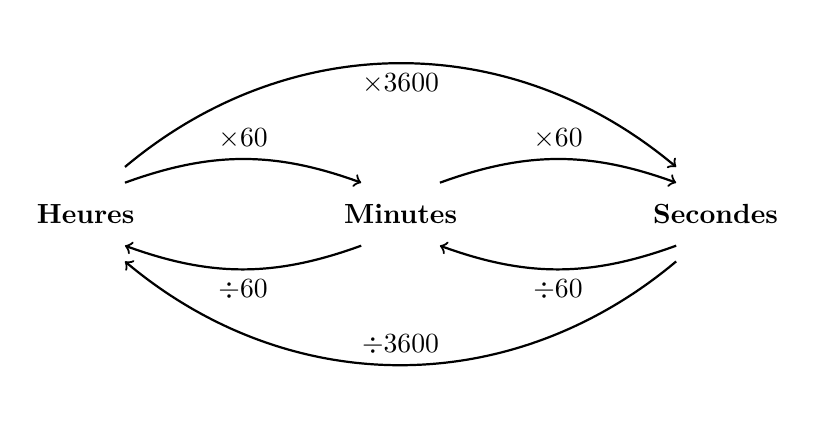
\begin{tikzpicture}[thick]
    
    % Labels des unités
    \node at (-4,0) {\textbf{Heures}};
    \node at (0,0) {\textbf{Minutes}};
    \node at (4,0) {\textbf{Secondes}};
    
    % Flèches et conversions vers la droite
    \draw[->, bend left=20] (-3.5,0.4) to node[above] {$\times 60$} (-0.5,0.4);
    \draw[->, bend left=20] (0.5,0.4) to node[above] {$\times 60$} (3.5,0.4);
    \draw[->, bend left=40] (-3.5,0.6) to node[below] {$\times 3600$} (3.5,0.6);
    
    % Flèches et conversions vers la gauche
    \draw[->, bend left=20] (-0.5,-0.4) to node[below] {$\div 60$} (-3.5,-0.4);
    \draw[->, bend left=20] (3.5,-0.4) to node[below] {$\div 60$} (0.5,-0.4);
    \draw[->, bend left=40] (3.5,-0.6) to node[above] {$\div 3600$} (-3.5,-0.6);
\end{tikzpicture}
\end{center}


\begin{Exemple} 
\vspace{-0.5cm}
\begin{minipage}[c]{0.7\textwidth}
Convertir 367 min en heures et minutes.\\
Comme 1 h = 60 min, on effectue une division euclidienne par 60. \\
Donc 367 min = {\color{Couleur8}\textbf{6}} h {\color{Couleur7}\textbf{7}} min.

\end{minipage} \hfill \begin{minipage}[c]{0.3\textwidth}
\begin{center}
\Division[CouleurCadre=white,Solution,CouleurSolution=black]{367}{60}
\end{center}
\end{minipage}

\end{Exemple}




\begin{Exemple}
\vspace{-1cm}
\begin{minipage}[c]{0.45\textwidth}
Convertir 34 990 s en heures, minutes et secondes. \\
On effectue \textbf{deux} divisions euclidiennes par 60 : \\
Donc 34 990 s = {\color{Couleur8}\textbf{583}} min {\color{Couleur7}\textbf{10}} s \\
\hspace*{2.5cm} = {\color{Couleur11}\textbf{9}} h {\color{Couleur12}\textbf{43}} min {\color{Couleur7}\textbf{10}} s.
\end{minipage} \hfill \begin{minipage}[c]{0.25\textwidth}
\begin{center}
\Division[CouleurCadre=white,Solution,CouleurSolution=black]{34990}{60}
\end{center}
\end{minipage} \hfill \begin{minipage}[c]{0.25\textwidth}
\begin{center}
\Division[CouleurCadre=white,Solution,CouleurSolution=black]{583}{60}
\end{center}
\end{minipage}

\end{Exemple}

\begin{Exemple}
Convertir 2 h 10 min 15 s en secondes.
\begin{itemize}[label=\textcolor{Couleur8}{$\bullet$}]
\item 2 h = 2 $\times$ 3 600 s = 7 200 s
\item 10 min = 10 $\times$ 60 s = 600 s
\item 2 h 10 min 15 s = 7 200 s + 600 s + 15 s = 7 815 s
\end{itemize}
\end{Exemple}

\begin{Exemple}
\begin{minipage}[c]{0.7\textwidth}
Convertir 5 h 12 min en heure décimale.
\begin{itemize}[label=\textcolor{Couleur8}{$\bullet$}]
\item Conversion des min en h : 12 min = 0,2 h
\item 5 h 12 min = 5,2 h
\end{itemize}
\end{minipage} \hfill \begin{minipage}[c]{0.25\textwidth}
\begin{center}
\DivisionD[CouleurCadre=white,Solution,CouleurSolution=black]{12}{60}
\end{center}
\end{minipage}

\end{Exemple}

\newpage 

\subsection*{II. Résoudre des problèmes avec des durées}
\addcontentsline{toc}{subsection}{II. Résoudre des problèmes avec des durées}

\begin{Exemple} 
Timothé arrive au collège à 8h32 et le quitte à 16h07. \\
Combien de temps est-il resté au collège ? \\
\begin{minipage}[c]{0.4\textwidth}
$ $ \\
\begin{itemize}[label=\textcolor{Couleur8}{$\bullet$}]
\item De 8h32 à 9h00 : 28 min
\item De 9h00 à 16h07 : 7 h 07 min
\item 28 min + 7 h 07 min = 7 h 35 min
\end{itemize} \vspace{0.5cm}
Timothé est resté 7 h 35 min au collège. 
\end{minipage} \hfill \begin{minipage}[c]{0.6\textwidth}
\begin{center}
\begin{tikzpicture}[thick]
    % Première boîte
    \draw[rounded corners,Couleur8, fill=Couleur8!20] (0,0.4) rectangle (1.5,1.2);
    \node at (0.75,0.8) {\textcolor{Couleur8}{\textbf{8 h 32}}};
    
    % Première flèche avec addition
    \draw[->, Couleur8, very thick] (1.5,0.8) -- (2.5,0.8);
    \node[Couleur8] at (2,1.6) {$+ 28$ min};
    
    % Première boîte intermédiaire (pointillés)
    \draw[dashed, Couleur8] (2.5,0.4) rectangle (4,1.2);
    \node[Couleur8] at (3.25,0.8) {\textbf{9 h}};
    
    % Deuxième flèche avec addition
    \draw[->, Couleur8, very thick] (4,0.8) -- (5,0.8);
    \node[Couleur8] at (4.5,1.6) {$+ 7$ h};
    
    % Deuxième boîte intermédiaire (pointillés)
    \draw[dashed, Couleur8] (5,0.4) rectangle (6.5,1.2);
    \node[Couleur8] at (5.75,0.8) {\textbf{16 h}};
    
    % Troisième flèche avec addition
    \draw[->, Couleur8, very thick] (6.5,0.8) -- (7.5,0.8);
    \node[Couleur8] at (7,1.6) {$+ 7$ min};
    
    % Boîte finale
    \draw[rounded corners,Couleur8, fill=Couleur8!20] (7.5,0.4) rectangle (9.5,1.2);
    \node at (8.5,0.8) {\textcolor{Couleur8}{\textbf{16 h 07}}};
\end{tikzpicture}
\end{center}\end{minipage}

\end{Exemple}


\begin{Exemple} 
Nour a roulé en vélo pendant 1 h 35 min. Elle est rentrée chez elle à 14h11. \\
A quelle heure était-elle partie ? \\
\begin{minipage}[c]{0.4\textwidth}
$ $ \\
\begin{itemize}[label=\textcolor{Couleur8}{$\bullet$}]
\item 14h11 - 11 min = 14h
\item 14h00 - 1h = 13h00
\item 13h00 - 24 min = 12h36
\end{itemize} \vspace{0.5cm}
Nour est partie à 12h36. 
\end{minipage} \hfill \begin{minipage}[c]{0.6\textwidth}
\begin{center}
\begin{tikzpicture}[thick]
    % Première boîte
    \draw[rounded corners,Couleur8, fill=Couleur8!20] (-0.5,0.4) rectangle (1.5,1.2);
    \node at (0.5,0.8) {\textcolor{Couleur8}{\textbf{12 h 36}}};
    
    % Première flèche avec addition
    \draw[->, Couleur8, very thick] (2.5,0.8) -- (1.5,0.8);
    \node[Couleur8] at (2,1.6) {$-24$ min};
    
    % Première boîte intermédiaire (pointillés)
    \draw[dashed, Couleur8] (2.5,0.4) rectangle (4,1.2);
    \node[Couleur8] at (3.25,0.8) {\textbf{13 h}};
    
    % Deuxième flèche avec addition
    \draw[->, Couleur8, very thick] (5,0.8) -- (4,0.8);
    \node[Couleur8] at (4.5,1.6) {$-1 $ h};
    
    % Deuxième boîte intermédiaire (pointillés)
    \draw[dashed, Couleur8] (5,0.4) rectangle (6.5,1.2);
    \node[Couleur8] at (5.75,0.8) {\textbf{14 h}};
    
    % Troisième flèche avec addition
    \draw[->, Couleur8, very thick] (7.5,0.8) -- (6.5,0.8);
    \node[Couleur8] at (7,1.6) {$-11$ min};
    
    % Boîte finale
    \draw[rounded corners,Couleur8, fill=Couleur8!20] (7.5,0.4) rectangle (9.5,1.2);
    \node at (8.5,0.8) {\textcolor{Couleur8}{\textbf{14 h 11}}};
\end{tikzpicture}
\end{center}\end{minipage}

\end{Exemple}


\begin{Exemple} 
Une évaluation a commencé à 9h43 et le premier élève l'a terminée au bout de 29 minutes. \\
A quelle heure a-t-il terminé ? \\
\begin{minipage}[c]{0.4\textwidth}
$ $ \\
\begin{itemize}[label=\textcolor{Couleur8}{$\bullet$}]
\item De 9h43 à 10h00 : 17 min
\item 10h00 + 12 min = 10h12.
\end{itemize} \vspace{0.5cm}
Il a terminé l'évaluation à 10h12.
\end{minipage} \hfill \begin{minipage}[c]{0.6\textwidth}
\begin{center}
\begin{tikzpicture}[thick]
    % Première boîte
    \draw[rounded corners,Couleur8, fill=Couleur8!20] (0,0.4) rectangle (1.5,1.2);
    \node at (0.75,0.8) {\textcolor{Couleur8}{\textbf{9 h 43}}};
    
    % Première flèche avec addition
    \draw[->, Couleur8, very thick] (1.5,0.8) -- (4,0.8);
    \node[Couleur8] at (2.75,1.6) {$+ 17$ min};
    
    % Première boîte intermédiaire (pointillés)
    \draw[dashed, Couleur8] (4,0.4) rectangle (5.5,1.2);
    \node[Couleur8] at (4.75,0.8) {\textbf{10 h}};
    
    % Deuxième flèche avec addition
    \draw[->, Couleur8, very thick] (5.5,0.8) -- (8,0.8);
    \node[Couleur8] at (6.75,1.6) {$+12$ min};
    

    % Boîte finale
    \draw[rounded corners,Couleur8, fill=Couleur8!20] (8,0.4) rectangle (10,1.2);
    \node at (9,0.8) {\textcolor{Couleur8}{\textbf{10 h 12}}};
    

\end{tikzpicture}
\end{center}
\end{minipage}

\end{Exemple}

